\section{Juego de la vida y Regla de Difusion}
  \paragraph{
  	Un Autómata es una máquina capaz de realizar determinadas operaciones o movimientos y pretende emular o sustituir comportamiento ya sea humano, natural o bajo criterios definidos.
  }
  \paragraph{
  	El concepto de Autómata es algo de suma importancia para el análisis de sistemas complejos. Uno de los sistemas complejos más conocidos y usados por su facilidad de implementación y diversas estructuras encontradas es el \textbf{Juego de la Vida} diseñado por el matemático John Conway en los años 70.
  }

  \paragraph{
  	El juego se desarrolla sobre una matriz cuadrada de filas y columnas infinitas (se parte del principio matemático), que se encuentra regido bajo reglas como nacimiento, supervivencia o muerte. Lo fascinante de este autómata es que considerando las reglas mencionadas se desarrollan con el paso de las generaciones patrones muy complejos o detallados, mostrando interacción o bien estabilidad en éstos.
  }
  \paragraph{
  	La regla de difusión, toma el principio de un autómata (tomando como base la estructura del juego de la vida). Sin embargo, cambia sus valores de nacimiento y muerte, también es conocida como la regla 2277, publicada en el año 2006 por el doctor Genaro Juárez en coolaboración Andrew Adamatzky y Harold V.McIntosh.
  }
  \paragraph{
  	La regla 2277, muestra patrones complejos además de un crecimiento o decaimiento mayor en la densidad de población a manejar dentro de la matriz del automata. Esto trae consigo información semejantes mas no identicas a las vista en el juego de la vida.
  }
  \clearpage
\section{Desarrollo, Implementación y Conclusiones} 
\subsection{Desarrollo e Implementación} 
	\paragraph{Se implementaron ambos automatas utilizando el paradigma de la programación orientada objetos y el uso de tecnologías basadas en la máquina virtual de java. Además se utilizó un control de versines como Git en conjunto con Github y un generador de projectos como Gradle.}
	\paragraph{
		Todo el código fuente puede ser encontrado en http://www.github.com/jresendiz27/ComplexSystems
	}
	\paragraph{
		Tomando como base esas tecnologías se fue aumentando la funcionalidad de la practica añadiendo el proceso de exploración del juego de la vida y la regla de difusión considerando un tamaño de matriz de 3x3, 4x4 y 5x5 respectivamente para cada una de estas.
	}
	\paragraph{
		Para poder almacenar la gran cantidad de información generada por el proceso de exploración se decidió usar MongoDB como gestor de documentos no relacionales, esto debido a su practico manejo de la información y el soporte de grandes bases.
	}
\subsection{Conclusiones}
	\paragraph{
		La creación de un simulador y la implementación de un proceso de exploración es algo que me cautivó como alumno a seguir mejorando y abriendo mi mente a nuevas ideas y tecnologías. 
	}
	\paragraph{
		Una de las desventajas vistas fue la tecnología usada, obstaculo que se trató de solventar con aplicación de diversas estructuras de datos y parametros enviados a la máquina virtual de Java.
	}
	\paragraph{
		Para el proceso de exploración se optó por generar todo el universo de posibilidades de forma concurrente y almacenarlas en una base no relacional, posteriormente se procedió a la busqueda de la información con base en un nodo que tenía una única referencia, generando así el grafo que muestra los estados del automata.
	}
	\paragraph{
		A continuación se muestran algunas capturas de pantalla de los procesos y simulación realizados:
	}
	\begin{figure}[h!]
      \centering
      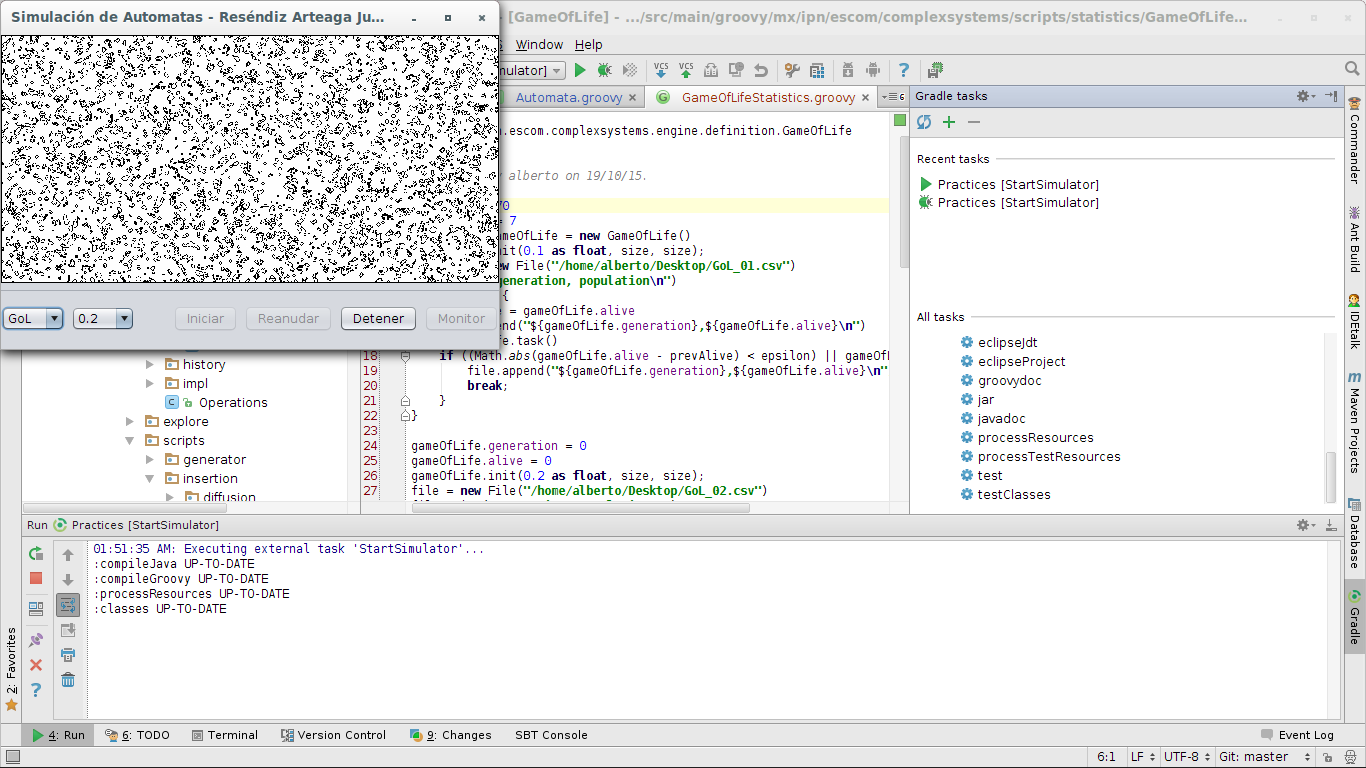
\includegraphics[width=15.5cm,height=11cm]{./images/simulador.png}
      \caption{Simulación}
    \end{figure}

    \begin{figure}[h!]
      \centering
      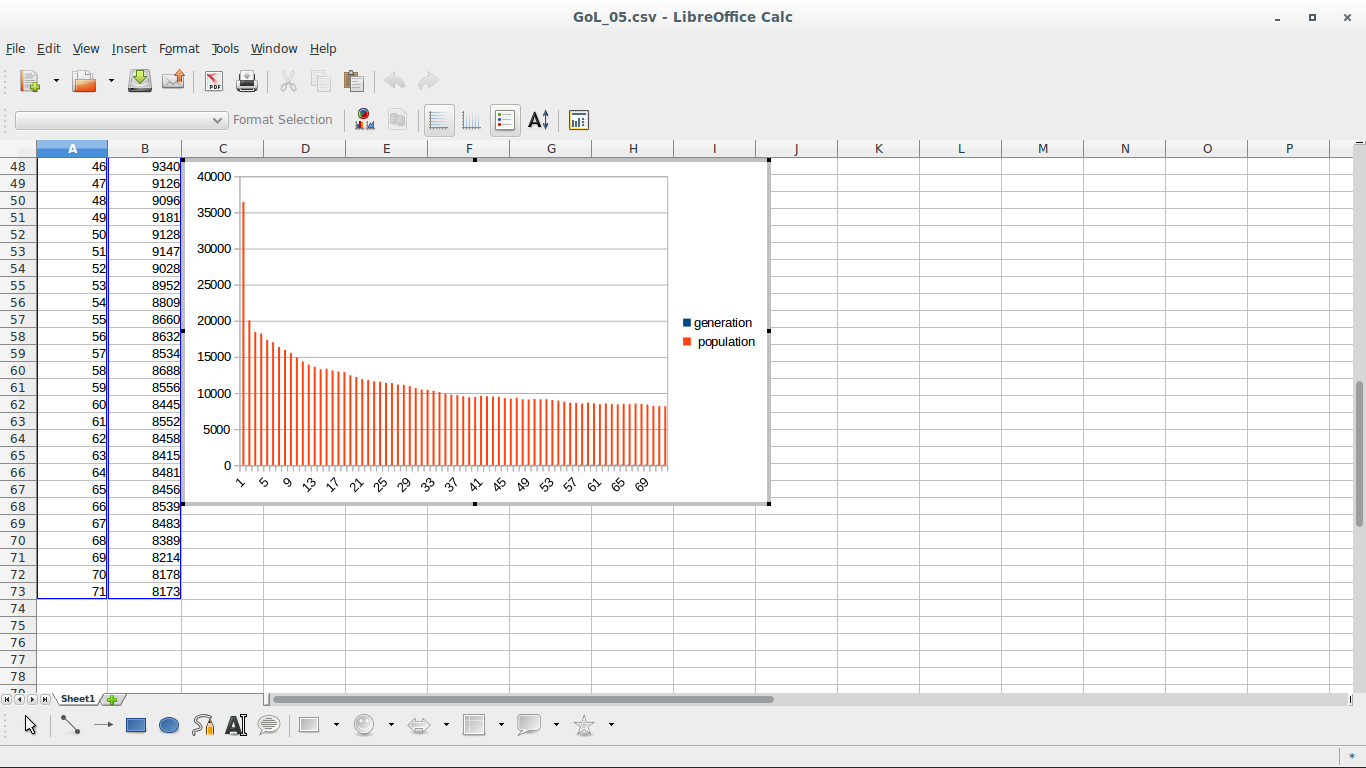
\includegraphics[width=15.5cm,height=11cm]{./images/densidades.png}
      \caption{Densidades}
    \end{figure}